%LogicFunctions.tex

\subsubsection{General considerations}
The heart of the simulation is the function \textit{logicFunction.m}, which determines the path any agent will choose to get to the other side of the hallway. To be more precise, it determines only the next step an agent will take and not the whole path. It relies heavily on the two functions \textit{xValuesLogic.m} to deal with other agents and \textit{xWallLogic.m} to deal with agents representing the wall or static obstacles. At first, the functioning of \textit{xValuesLogic.m} will be explained and afterwards the functioning of \textit{xWallLogic}.\\

\subsubsection{How to get $\beta_\y{Links}$ and $\beta_\y{Rechts}$?}
\begin{figure}[h!]
	\centering
		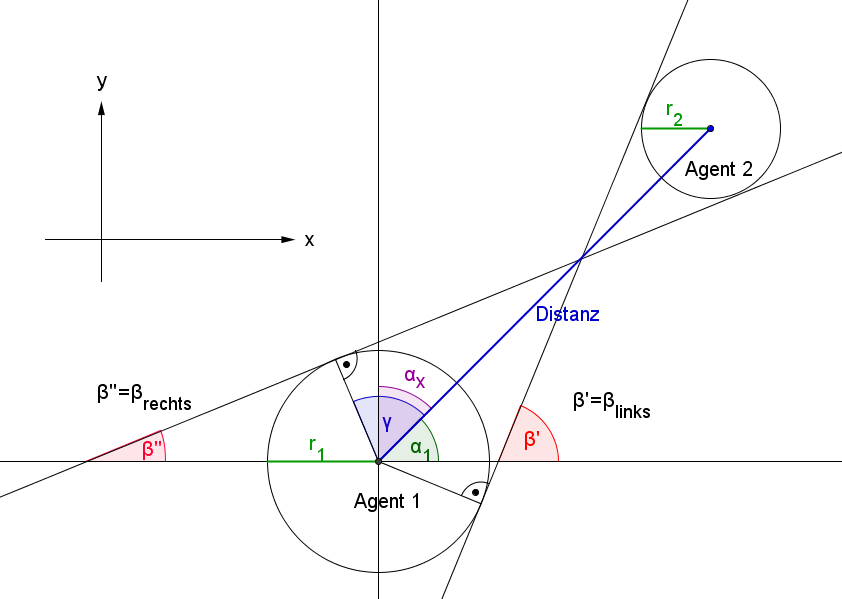
\includegraphics[width=0.80\textwidth]{pictures/beta.PNG}
	\caption{The graph shows the angles and variables used to get $\beta_\y{Links}$ and $\beta_\y{Rechts}$. $\alpha_X$ is the angle between the two agents with respect to the $y$-axis. This depiction was engineered to work also for agents walking the other way.}
	\label{fig:beta}
\end{figure}

\noi For our model, it is crucial to determine where an agent shouldn't go. The function \textit{getBeta.m} returns the angles which describe the interval leading to a collision. A graphical depiction of the situation is given in figure \ref{fig:beta}. The equations (\ref{logik3}) to (\ref{logik5}) were used to get $\beta_\y{Links}$ and $\beta_\y{Rechts}$. They had to be converted into the angles given with respect to $\varphi$, $\beta_{\varphi,\y{ left}}$ and $\beta_{\varphi,\y{ right}}$ as shown in equations (\ref{logik6}) to (\ref{logik7}).
\begin{equation}\label{logik3}
	\gamma = arccos\brac{\frac{r_S}{d}},\ \alpha = arctan\brac{\frac{\Delta y}{\Delta x}}
\end{equation}
\begin{equation}\label{logik4}
	\beta_\y{Links} = \gamma + \alpha - \frac{\pi}{2}
\end{equation}
\begin{equation}\label{logik5}
	\beta_\y{Rechts} = + \alpha + \frac{\pi}{2} - \gamma
\end{equation}
\begin{equation}\label{logik6}
  \beta_{\varphi,\y{ left}} = \frac{\pi}{2} - \beta_\y{Rechts} = \pi - (\gamma + \alpha)
\end{equation}
\begin{equation}\label{logik7}
  \beta_{\varphi,\y{ right}} = \frac{\pi}{2} - \beta_\y{Rechts} = \gamma - \alpha)
\end{equation}
\noi This works between agents as well as between agents and the wall agents. Care was taken to engineer a calculation that allows for it to be used for agents walking in both directions.

\subsubsection{xValuesLogic.m}
\text{xValuesLogic.m} distinguishes three different cases.
\begin{itemize}
	\item For two crossing agents, we used equation (\ref{logik1}) to get $x_\y{out}'$. 
	\begin{equation}\label{logik1}
		x_\y{out}' = \frac{1}{\dis (|x - \alpha_X|)^{\brac{\frac{-\Delta v}{a}}}} = (|x - \alpha_X|)^{\brac{\frac{\Delta v}{a}}},\ \Delta v < 0
	\end{equation}
	\noi All values which correspond to a collision course in $x_y{out}'$ are set to zero. This also deals with the singularity of equation (\ref{logik1}) as it is set to zero. Afterwards, $x_\y{out}'$ is normalized and modificated further using equation (\ref{logik2}).
	\begin{equation}\label{logik2}
		x_\y{out} = x_\y{out}' \cdot \frac{b}{max(x_\y{out}')} \cdot \brac{\frac{r_S}{d}}^c
	\end{equation}
	\noi The variables $a$ (called \textit{SLOPEFACTOR}), $b$ (\textit{HEIGHT}) and $c$ (\textit{REPULSIONAGENT}) have to chosen in a way that the simulation runs smoothly. The term $\frac{b}{max(x_\y{out}')}$ normalized the function to a maximum value $b$ while the term $\brac{\frac{r_S}{d}}^c$ controls that the repulsive influence gets stronger the closer the two agents get. $c$ is usually chosen to be larger than 1.


